\begin{figure}[htpb]
\begin{center}
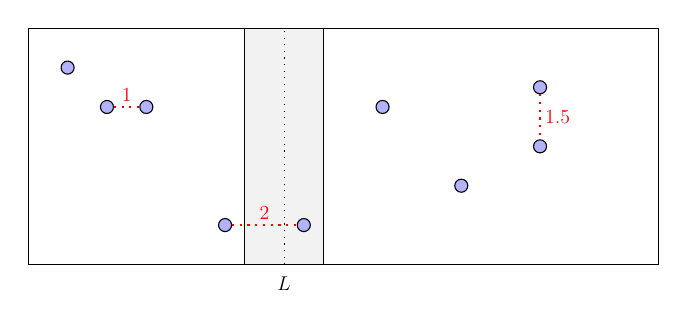
\begin{tikzpicture}[scale=0.5, transform shape]
	\draw (-8,-3) rectangle (8,3);

	\only<2->{
		\draw[fill=gray!10] (-2.5,-3) rectangle (-0.5,3);
	}
	\foreach \x/\y/\name in {
		-7/2/,
		-6/1/l1,
		-5/1/l2,
		-3/-2/c1,
		-1/-2/c2,
		3/-1/,
		5/1.5/r1,
		5/0/r2,
		}{
		\node[circle, black, draw, fill=blue!30, minimum size=4pt] (\name) at (\x,\y) {};
	}
		\draw[dotted] (-1.5,-3) -- (-1.5,3);
		\node at (-1.5, -3.5) {\Large $L$};
		\draw[dotted, red, thick] (l1) --  node[anchor=south] {\Large 1} (l2);
		\draw[dotted, red, thick] (r1) --  node[anchor=west] {\Large 1.5} (r2);
		\draw[dotted, red, thick] (c1) --  node[anchor=south] {\Large 2} (c2);

\end{tikzpicture}
\end{center}
\end{figure}
